% Foliensatz: "AFu-Kurs nach DJ4UF" von DK0TU, Amateurfunkgruppe der TU Berlin
% Lizenz: CC BY-NC-SA 3.0 de (http://creativecommons.org/licenses/by-nc-sa/3.0/de/)
% Autoren: Felix Baum DB4UM <baum@campus.tu-berlin.de>
% Korrekturen: Lars Weiler <dc4lw@darc.de>
% Review: DL7BST

\documentclass[aspectratio=169]{beamer}

\usepackage[ngerman]{babel} % deutsche Worttrennung etc.
\usepackage[utf8]{inputenc} % UTF8 Text

\usepackage[super, comma, numbers, square, sort]{natbib}

\usepackage{hyperref}       % Hyperref Package für bessere Referenzen (todo)
\hypersetup{
	colorlinks=false,       %   false: boxed links; true: colored links
    %linkcolor=white,       %   color of internal links (change box color with linkbordercolor)
    citecolor=red,          %   color of links to bibliography
    filecolor=white,        %   color of file links
    urlcolor=blue           %   color of external links
}

\usepackage{multirow}
\usepackage{wasysym}  % Math Symbols like \permil
%\usepackage{colortbl}
%\usepackage{subscript}
%\usepackage{caption}
%\usepackage{setspace}
%\usepackage{xcolor}        % benutze CodeListe

% Footnote
%\usepackage{hanging}
%
%\setbeamertemplate{footnote}{%
%  \hangpara{2em}{1}%
%  \makebox[2em][l]{\insertfootnotemark}\footnotesize\insertfootnotetext\par%
%}


%\usepackage{pgf}
%\usepackage{tikz}
%\usetikzlibrary{arrows,automata}
%\usetikzlibrary{positioning}
%
%\tikzset{
%    state/.style={
%           rectangle,
%           rounded corners,
%           draw=black, very thick,
%           minimum height=2em,
%           minimum width=2pt,
%           inner sep=2pt,
%           text centered,
%           },
%}

%\usepackage{listings}
%\lstset{basicstyle=\small, numberstyle=\tiny, extendedchars=true, numbers=left, numbersep=5pt}
%\lstset{showtabs=false, showspaces=false, showstringspaces=false}
%%\lstset{backgroundcolor=\color{white!75!lightgray}, , frame=single}
%%\lstset{backgroundcolor=\color{white}}
%%\lstset{backgroundcolor=none}
%\lstset{keywordstyle=\color{blue!50!gray},  identifierstyle=\color{black}}
%\lstset{commentstyle=\color{green!50!gray}, stringstyle=\color{red!50!gray}}
%\lstset{language=C, fontadjust=true, tabsize=2, breaklines=true}
%\lstset{backgroundcolor=\color{white!75!lightgray}, caption=\lstname, frame=single}
%\lstset{emphstyle=\color{black}\fbox}
%
%% Keine "Listing:"-Caption
%\captionsetup{labelformat=empty,labelsep=none}
%
%% für mathematische Umgebungen
%\usepackage{amsmath,amsfonts,amssymb}
%
%\lstdefinestyle{Bash}{
%language=Bash,
%frame=single,
%rulecolor=\color{black},
%backgroundcolor=\color{gray!50},
%keywordstyle=\color{black},
%identifierstyle=,
%commentstyle=\color{black},
%stringstyle=\color{magenta!65!white},
%showstringspaces=false,
%basicstyle=\footnotesize\ttfamily\color{black},
%numbers=none,
%breaklines=true,
%captionpos=b
%}

%\usepackage{listings}
%
%\lstdefinestyle{basic}{
%    captionpos=t,%
%    basicstyle=\footnotesize\ttfamily,%
%    numberstyle=\tiny,%
%    numbers=left,%
%    stepnumber=1,%
%    frame=single,%
%    showspaces=false,%
%    showstringspaces=false,%
%    showtabs=false,%
%    %
%    keywordstyle=\color{blue},%
%    identifierstyle=,%
%    commentstyle=\color{gray},%
%    stringstyle=\color{magenta}%
%}



% fließende Boxen haben keinen Abstand
%\fboxsep0mm

% inkludiere Creative Commons Helper
%%%%%%%%%%%%%%%%%%%%%%%%%%%%%%%%%%%%%%%%%%%%%%%%%%%%%%%%%%%%%%%%
%% ccBeamer 0.1, 2007-07-02                                   %%
%% Written by Sebastian Pipping <webmaster@hartwork.org>      %%
%% ---------------------------------------------------------- %%
%% Licensed under Creative Commons Attribution-ShareAlike 3.0 %%
%% http://creativecommons.org/licenses/by-sa/3.0/             %%
%%%%%%%%%%%%%%%%%%%%%%%%%%%%%%%%%%%%%%%%%%%%%%%%%%%%%%%%%%%%%%%%


%% Images
\newcommand{\CcImageBy}[1]{%
	
\includegraphics[scale=#1]{texdata/creative_commons/cc_by_30.pdf}%
}
\newcommand{\CcImageCc}[1]{%
	
\includegraphics[scale=#1]{texdata/creative_commons/cc_cc_30.pdf}%
}
\newcommand{\CcImageDevNations}[1]{%
	
\includegraphics[scale=#1]{texdata/creative_commons/cc_dev_nations_30.pdf}%
}
\newcommand{\CcImageNc}[1]{%
	
\includegraphics[scale=#1]{texdata/creative_commons/cc_nc_30.pdf}%
}
\newcommand{\CcImageNd}[1]{%
	
\includegraphics[scale=#1]{texdata/creative_commons/cc_nd_30.pdf}%
}
\newcommand{\CcImagePd}[1]{%
	
\includegraphics[scale=#1]{texdata/creative_commons/cc_pd_30.pdf}%
}
\newcommand{\CcImageSa}[1]{%
	
\includegraphics[scale=#1]{texdata/creative_commons/cc_sa_30.pdf}%
}
\newcommand{\CcImageSampling}[1]{%
	
\includegraphics[scale=#1]{texdata/creative_commons/cc_sampling_30.pdf}%
}
\newcommand{\CcImageSamplingPlus}[1]{%
	
\includegraphics[scale=#1]{texdata/creative_commons/cc_sampling_plus_30.pdf}%
}


%% Groups
\newcommand{\CcGroupBy}[2]{% zoom, gap
	\CcImageCc{#1}\hspace*{#2}\CcImageBy{#1}%
}
\newcommand{\CcGroupByNc}[2]{% zoom, gap
	\CcImageCc{#1}\hspace*{#2}\CcImageBy{#1}\hspace*{#2}\CcImageNc{#1}%
}
\newcommand{\CcGroupByNcNd}[2]{% zoom, gap
	\CcImageCc{#1}\hspace*{#2}\CcImageBy{#1}\hspace*{#2}\CcImageNc{#1}\hspace*{#2}\CcImageNd{#1}%
}
\newcommand{\CcGroupByNcSa}[2]{% zoom, gap
	\CcImageCc{#1}\hspace*{#2}\CcImageBy{#1}\hspace*{#2}\CcImageNc{#1}\hspace*{#2}\CcImageSa{#1}%
}
\newcommand{\CcGroupByNd}[2]{% zoom, gap
	\CcImageCc{#1}\hspace*{#2}\CcImageBy{#1}\hspace*{#2}\CcImageNd{#1}%
}
\newcommand{\CcGroupBySa}[2]{% zoom, gap
	\CcImageCc{#1}\hspace*{#2}\CcImageBy{#1}\hspace*{#2}\CcImageSa{#1}%
}
\newcommand{\CcGroupDevNations}[2]{% zoom, gap
	\CcImageCc{#1}\hspace*{#2}\CcImageDevNations{#1}%
}
\newcommand{\CcGroupNcSampling}[2]{% zoom, gap
	\CcImageCc{#1}\hspace*{#2}\CcImageNc{#1}\hspace*{#2}\CcImageSampling{#1}%
}
\newcommand{\CcGroupPd}[1]{% zoom
	\CcImagePd{#1}%
}
\newcommand{\CcGroupSampling}[1]{% zoom
	\CcImageSampling{#1}%
}
\newcommand{\CcGroupSamplingPlus}[1]{% zoom
	\CcImageSamplingPlus{#1}%
}


%% Text
\newcommand{\CcLongnameBy}{Attribution}
\newcommand{\CcLongnameByNc}{Attribution-NonCommercial}
\newcommand{\CcLongnameByNcNd}{Attribution-NoDerivs}
\newcommand{\CcLongnameByNcSa}{Attribution-NonCommercial-ShareAlike}
\newcommand{\CcLongnameByNd}{Attribution-NoDerivs}
\newcommand{\CcLongnameBySa}{Attribution-ShareAlike}

\newcommand{\CcNote}[1]{% longname
	This work is licensed under the \textit{Creative Commons #1 3.0 License}.%
}


% generelles Thema auswählen
\usetheme{Goettingen} %Berlin spart ohne Sidebar allerdings angenehm Platz
% AnnArbor | Antibes | Bergen | Berkeley | Berlin | Boadilla | boxes | CambridgeUS | Copenhagen | Darmstadt | default | Dresden | Frankfurt | Goettingen | Hannover | Ilmenau | JuanLesPins | Luebeck | Madrid | Malmoe | Marburg | Montpellier | PaloAlto | Pittsburgh | Rochester | Singapore | Szeged | Warsaw

% Farben wählen
\usecolortheme{beetle}
% beaver | beetle | crane | default | dolphin | dove | fly | lily | orchid | rose | seagull | seahorse | sidebartab | structure | whale | wolverine

% Setze alle Farben auf Grau und Weiß
%\definecolor{craneorange}{RGB}{64,64,64}
%\definecolor{craneblue}{RGB}{255,255,255}

% Schriftart wählen
\usefonttheme{default}
% default | professionalfonts | serif | structurebold | structureitalicserif | structuresmallcapsserif

% Innere Themen(Kopf-, Fuß-, Sidebar usw)
%\useinnertheme{default}
\useinnertheme{circles}
% default | inmargin | rectangles | rounded | circles

% Äußere Themen (Anordnung der inneren, grenzen der Folien etc.)
\useoutertheme{infolines}
% default | infolines | miniframes | shadow | sidebar | smoothbars | smoothtree | split | tree

% Deaktiviere Navigations-Symbole ({} -> leer)
\setbeamertemplate{navigation symbols}{}
%\setbeamertemplate{navigation symbols}{\large \ifnum \insertframenumber <10 0\fi\insertframenumber/\inserttotalframenumber\vspace*{0.2ex}}

% Zeige ein Hintergrundbild
\setbeamertemplate{background canvas}{
        \hspace*{-2.0cm}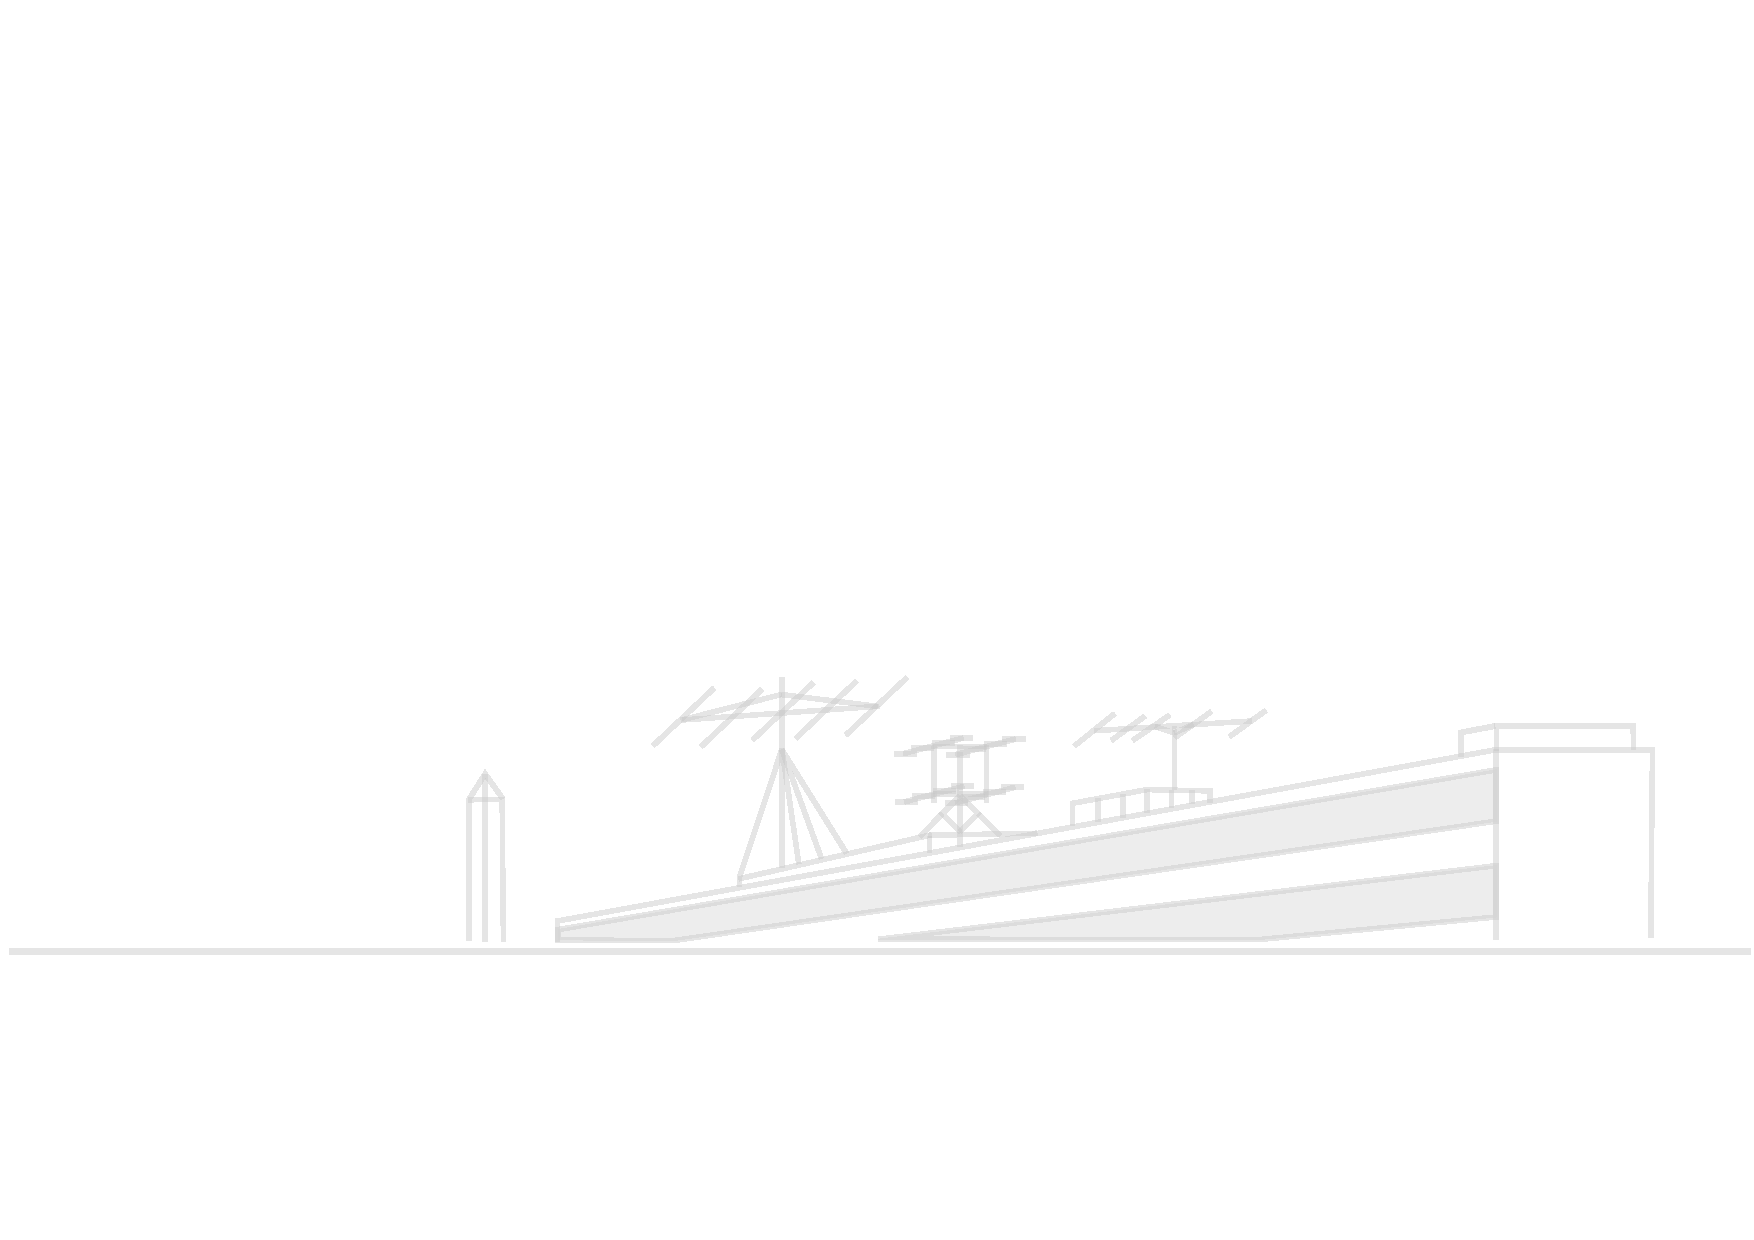
\includegraphics[width=17.8cm]{texdata/dk0tu_rooftop_background.pdf}
}

% Foliennummer einfügen
\setbeamertemplate{footline}[frame number]
%\setbeamertemplate{footline}{}

% Ändere das Zeichen vor jedem item
%\setbeamertemplate{itemize item}{\color{craneorange}$\blacktriangleright$}
%\setbeamertemplate{itemize subitem}{\color{craneorange}$\triangleright$}
%\setbeamertemplate{itemize subsubitem}{\color{craneorange}$\blacktriangleright$}

% Ändert die Blöcke 
\setbeamertemplate{blocks}[rounded][shadow=true]
% default | rounded [shadow=true|false]

%
% Eigene Kommandos
%

% Hack to get natbib and beamer working together. "The beamer user guide suggests
% that only the manual bibliography entry approach is supported"
% on some system it works out of the box, sometimes you need the hack :-(
% so check it --dl7bst
\ifdefined\newblock
    \relax
\else
    \newcommand{\newblock}{}
\fi

% \includedia command to generate png out of a dia file
% NEEDS installed dia and pdflatex option --shell-escape
\newcommand{\includedia}[1]{
    \immediate\write18{/usr/bin/dia #1.dia -e #1_diatmp.png -t png}
}

% RICHIG GROSSER FONT!
\newfont{\bigfont}{cmr10 at 144pt}
\newfont{\smallfont}{cmr10 at 8pt}

% Römische Ziffern
\makeatletter
\newcommand{\rmnum}[1]{\romannumeral #1}
\newcommand{\Rmnum}[1]{\expandafter\@slowromancap\romannumeral #1@}
\makeatother

% Schwarze Überschrift
%\setbeamercolor{frametitle}{fg=black}
%\setbeamercolor{title}{fg=black}

% Item- und Box-Farben
\definecolor{deepBlue}{HTML}{000066}
\setbeamercolor{itemize item}{fg=deepBlue}
\setbeamercolor{itemize subitem}{fg=deepBlue}
\setbeamercolor{description item}{fg=deepBlue}
\setbeamercolor{block title}{fg=deepBlue!100, bg=blue!15}
\setbeamercolor{block body}{fg=black, bg=blue!5}
\setbeamercolor{block title alerted}{fg=deepBlue, bg=red!75}
\setbeamercolor{block body alerted}{fg=black, bg=red!15}
\setbeamercolor*{block title example}{fg=blue!50, bg=blue!10}
\setbeamercolor*{block body example}{fg= blue, bg=blue!5}

%\setbeamercolor{section in head/foot}{parent=palette primary}
%\setbeamercolor{subsection in head/foot}{parent=palette secondary}
%\setbeamercolor{sidebar}{fg=darkblue,bg=yellow!90!orange}
%\setbeamercolor{title in sidebar}{fg=darkblue}
%\setbeamercolor{author in sidebar}{fg=darkblue}
%\setbeamercolor{section in sidebar}{fg=darkblue!10!black}
%\setbeamercolor{subsection in sidebar}{fg=darkblue!50!black}

% Titlepage Infos
\title{AFu-Kurs nach DJ4UF}
\author[DKØTU]{DKØTU\\ \footnotesize{Amateurfunkgruppe der TU Berlin}}
\institute[DKØTU]{\url{http://www.dk0tu.de} }

% PDF-Eigenschaften
\subject{DK0TU-Amateurfunkkurs nach DJ4UF}
\keywords{Amateurfunk Kurs HAM Radio Course CC-BY-NC-SA OpenSource TU Berlin DK0TU}

\subtitle{Technik A19: \\
            EMV und Sicherheit \\[2em]}
\date{Stand 12.07.2016}
 \begin{document}

\begin{frame}
    \titlepage
    \vfill
    \begin{center}
        \ccbyncsaeu\\
        {\tiny This work is licensed under the \em{Creative Commons Attribution-NonCommercial-ShareAlike 3.0 License}.}\\[0.5ex]
         \tiny Amateurfunkgruppe der Technische Universität Berlin (AfuTUB), DKØTU
         %\includegraphics[scale=0.5]{img/DK0TU_Logo.pdf}
    \end{center}
\end{frame}


\section*{Störungen}

\begin{frame}
    \frametitle{Funkwagen der Bundesnetzagentur}
    \begin{center}
		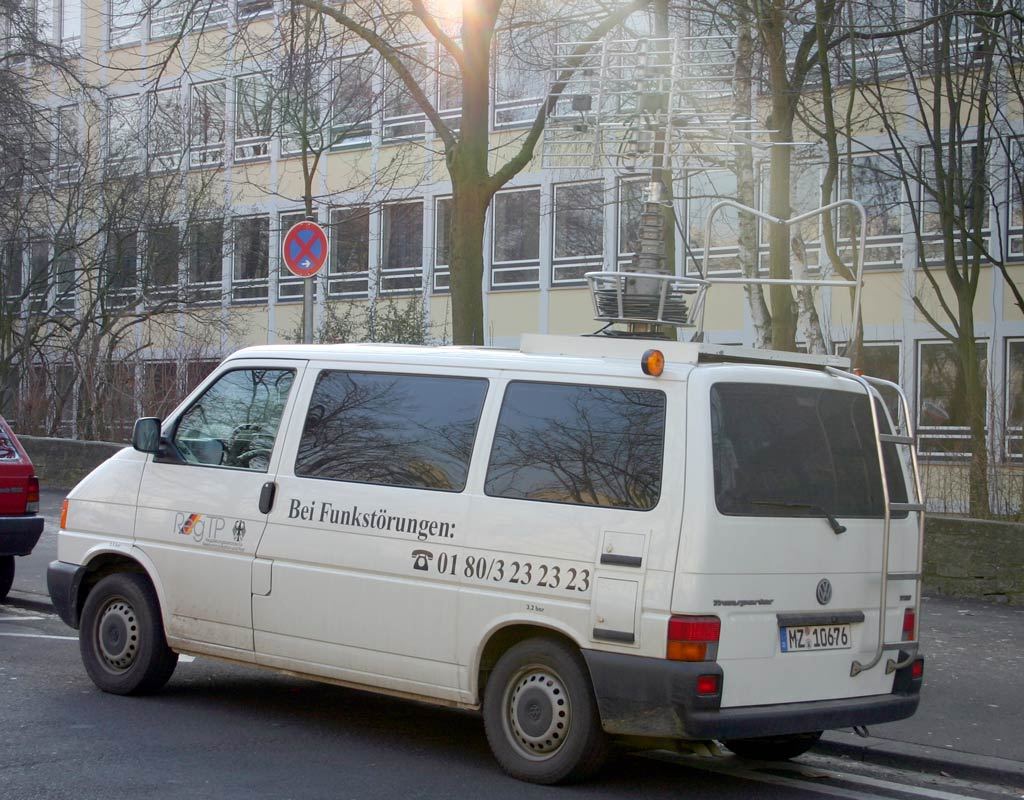
\includegraphics[width=1\textwidth,height=.85\textheight,keepaspectratio]{a19/FunkwagenBNetz.jpg}\\
    {\tiny \hyperlink{refs}{\cite{wm}} \\[1em]}
	\end{center}
\end{frame}

\begin{frame}
  \frametitle{Störung}
  \begin{center}
    \begin{block}{Verordnung zum Gesetz über den Amateurfunk (Amateurfunkverordnung -- AFuV) \\
      § 16 Technische und betriebliche Rahmenbedingungen für Amateurfunkstellen}
      (4) Unerwünschte Aussendungen sind auf das geringst mögliche Maß zu beschränken. Erforderliche Richtwerte für Funkanlagen nach § 1 Abs. 3 Nr. 1 des Gesetzes über Funkanlagen und Telekommunikationsendeinrichtungen vom 31.~Januar~2001 werden nach Anhörung der betroffenen Kreise im Amtsblatt der Regulierungsbehörde veröffentlicht.
    \end{block}
  \end{center}
\end{frame}

\begin{frame}
  \frametitle{Elektrisches Feld}
  \begin{center}
    \begin{block}{Grenzen für Geräte von Funkamateuren}
      \begin{tabular}{p{.21\textwidth}|p{.35\textwidth}|p{.35\textwidth}}
        Frequenzbereich & Erforderliche Dämpfung unerwünschter Aussendungen gegenüber der maximalen PEP des Senders & Alternativ maximal zulässige Leistung unerwünschter Aussendungen \\ \hline \hline
        150\,kHz--1,7\,MHz & $60dB$ & $0,25 \mu W$ \\ \hline
        1,7\,MHz--35\,MHz & $40dB$ & $0,25 \mu W$ \\ \hline
        35\,MHz--50\,MHz & $40dB + 129,1 \cdot log \frac{f}{35}dB $ & $0,25 \mu W$ \\ \hline
        50\,MHz--1\,GHz & $60dB$ & $0,25 \mu W$ \\ \hline
        1GHz--40\,GHz & $50dB$ & $1 \mu W$
      \end{tabular}
    \end{block}
  \end{center}
\end{frame}

\begin{frame}
  \frametitle{Oberwelle}
  \begin{center}
    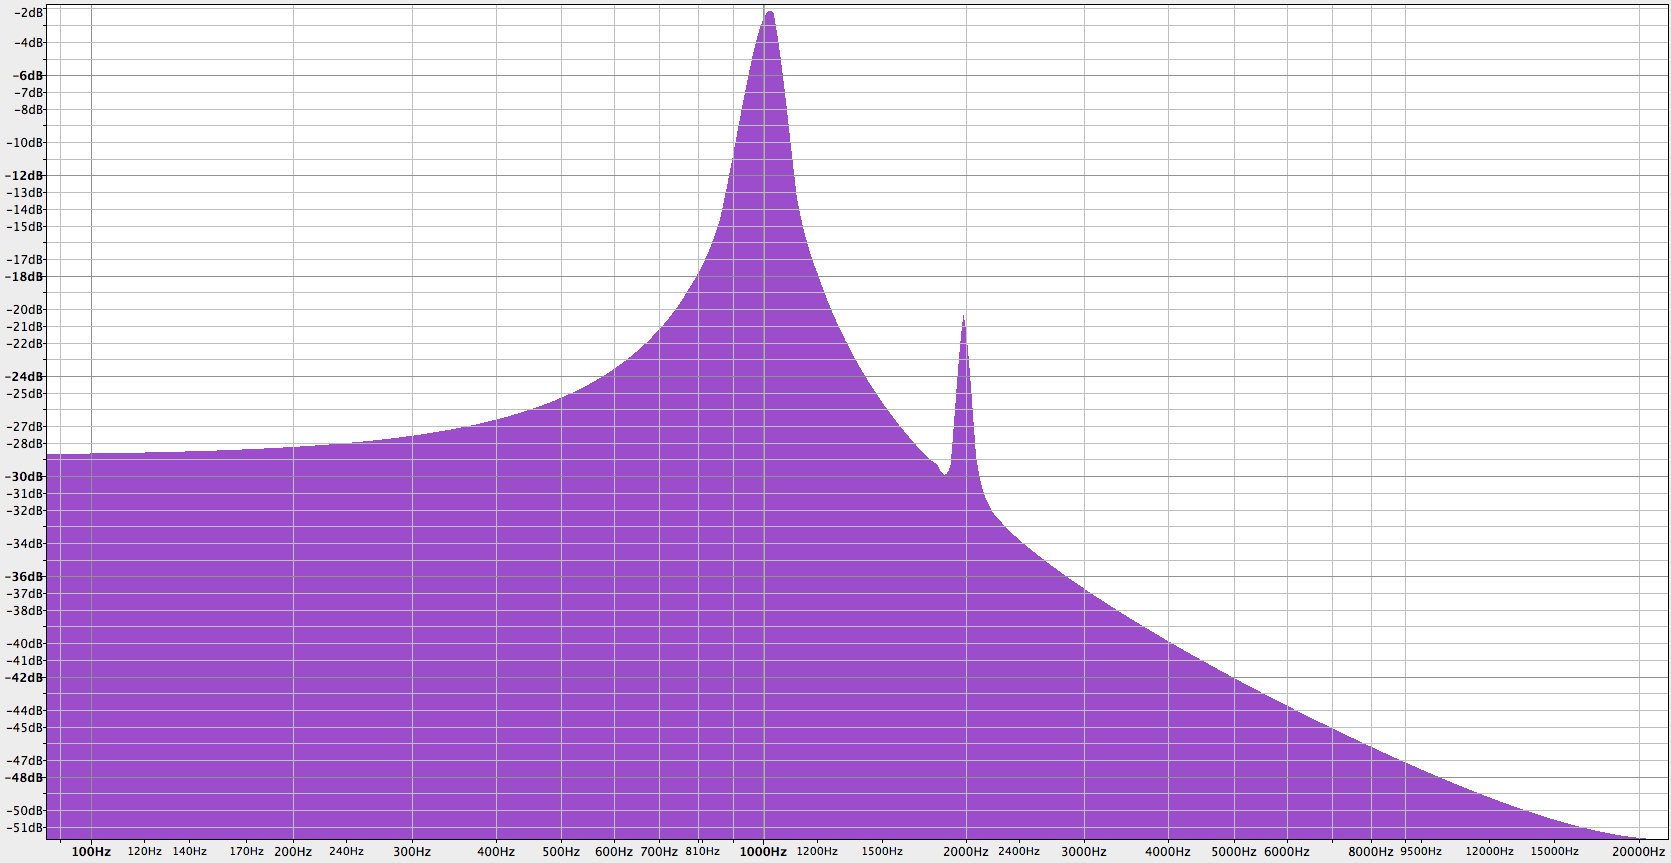
\includegraphics[width=1\textwidth,height=.80\textheight,keepaspectratio]{a19/oberwelle.png}\\
    {\tiny von DB4UM mit Audacity}
  \end{center}
\end{frame}

\begin{frame}
  \frametitle{Oberwelle}
  \begin{center}
    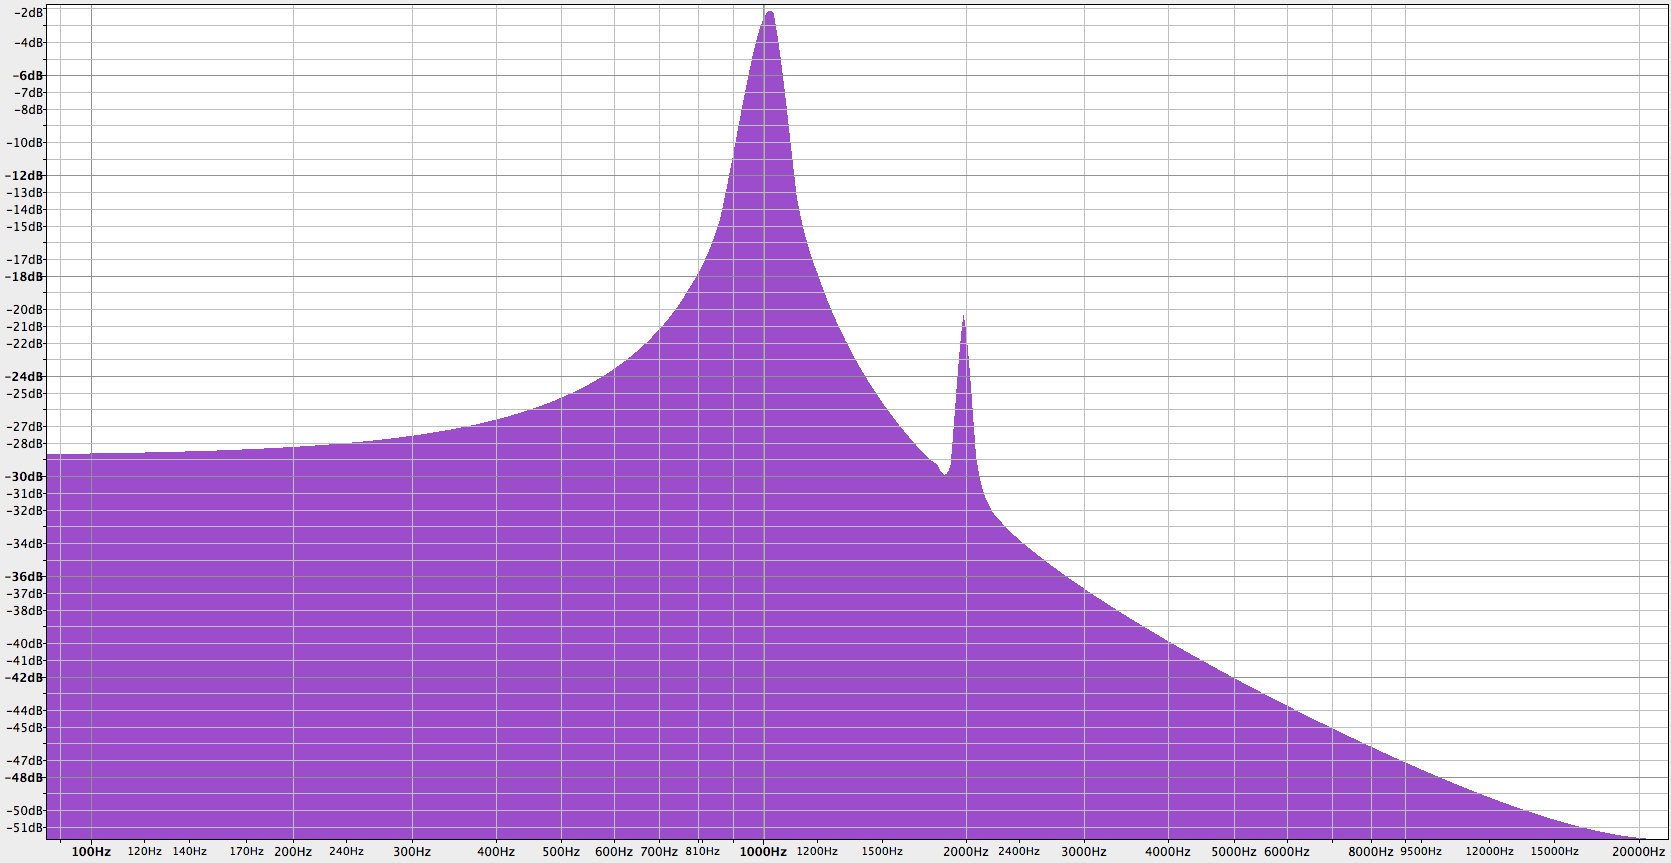
\includegraphics[width=0.8\textwidth,height=.65\textheight,keepaspectratio]{a19/oberwelle.png}\\[2em]
    Abhilfe bei zu starken Oberwellen schafft ein Tiefpass oder noch besser ein Bandpassfilter.
  \end{center}
\end{frame}

\begin{frame}
  \frametitle{Störung -- Bandgrenzen}
  \begin{center}
    \begin{block}{Senden innerhalb der Bandgrenzen}
      Beim Funken ist immer auf die Bandgrenzen zu achten. So ist z.B. SSB $3kHz$ breit und oberhalb der eingestellten Frequenz. Ist also bei $14,350MHz$ das Band zu Ende darf dort mit SSB nur bis $14,347MHz$ gesendet werden.
    \end{block}
  \end{center}
\end{frame}

\section*{EMV}

\begin{frame}
  \frametitle{EMV Probleme}
  \begin{center}
    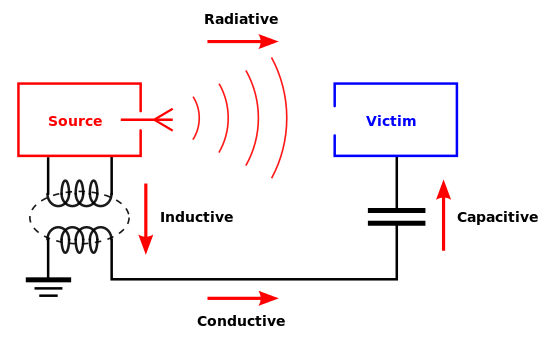
\includegraphics[width=1\textwidth,height=.85\textheight,keepaspectratio]{a19/EMI_coupling_modes.png}\\
    {\tiny \hyperlink{refs}{\cite{wm}}}
  \end{center}
\end{frame}

\begin{frame}
  \frametitle{EMV}
  \begin{center}
    \begin{block}{Einströmungen und Einstrahlungen}
      \begin{description}
        \item[Einströmung] Elektromagnetische Energie koppelt in die Kabel ein. \\
        \item[Einstrahlung] Elektromagnetische Energie koppelt direkt ins Gerät.
      \end{description}
    \end{block}
  \end{center}
\end{frame}

\begin{frame}
  \frametitle{EMV}
  \begin{center}
    \begin{exampleblock}{Einströmungen und Einstrahlungen}
      Ist das Knacken in den Lautsprechern, wenn das Handy daneben liegt, eine Einströmung oder eine Einstrahlung?
    \end{exampleblock}
  \end{center}
\end{frame}

\section*{Beseitigung von Störungen}

\begin{frame}
  \frametitle{Beseitigung von Störungen}
  \begin{center}
    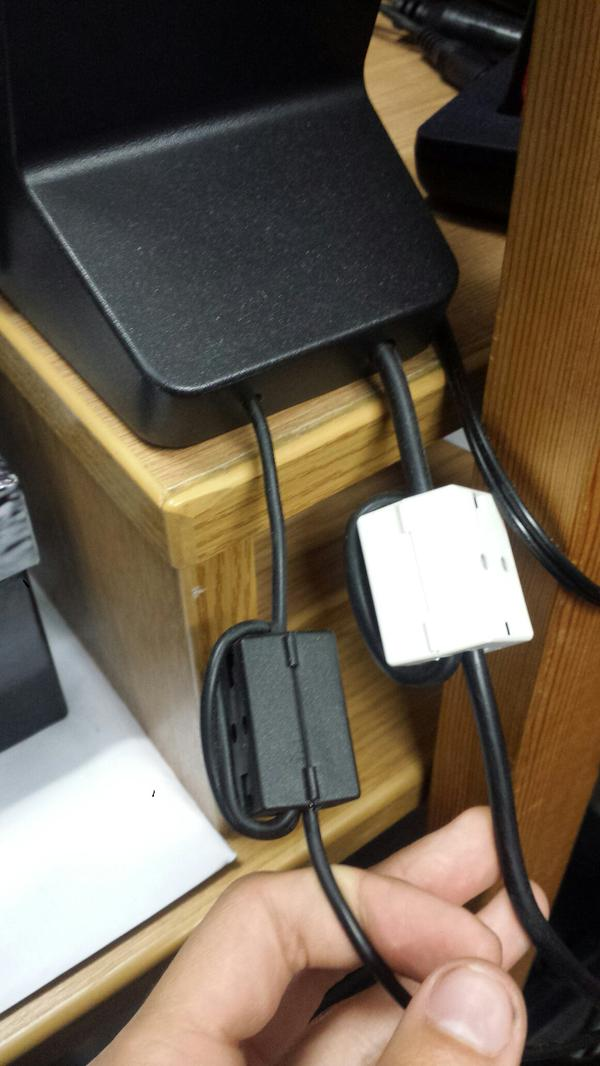
\includegraphics[width=\textwidth,height=0.80\textheight,keepaspectratio]{a19/2Filter.jpg}\\
    {\tiny Lautsprecher im Shack von DK0TU}
  \end{center}
\end{frame}

\begin{frame}
  \frametitle{Beseitigung von Störungen}
  \begin{center}
    \begin{block}{Ferrit zum Entstören als Mantelwellendrossel}
      Mit Klappferriten oder Ferritkernen können Kabel TP-gefiltert und somit von HF-Einstrahlung entstört werden. Seien es Lautsprecherkabel, Stromversorgung oder Datenkabel.
    \end{block}
    \begin{block}{Abblock-Kondensatoren}
      Innerhalb der Schaltung neben ICs und anderen Bauteilen, die eine stabile Gleichspannung benötigen, Abblock-Kondensatoren einbauen.
    \end{block}
  \end{center}
\end{frame}

\begin{frame}
  \frametitle{Beseitigung von Störungen}
  \begin{center}
    \begin{block}{Metallgehäuse gegen Einstrahlung}
      Oftmals sind auch innerhalb von HF-Schaltungen Schaltungsteile wie VHF Oszillatoren mit einem extra Metallkasten umgeben, um nicht in andere Schaltungsteile einzustrahlen. Das Gehäuse auf jeden Fall erden.
    \end{block}
  \end{center}
\end{frame}

\begin{frame}
  \frametitle{Beseitigung von Störungen}
  \begin{center}
    \begin{exampleblock}{TK119}
      Während einer ATV-Aussendung erscheint das Bild auch auf dem Fernsehgerät der Nachbarn. Eine mögliche Abhilfe der Störung wäre die \ldots \\[3em]
      \only<1>{\vspace{1em}}
      \only<2>{\ldots Verminderung der Ausgangsleistung.}
    \end{exampleblock}
  \end{center}
\end{frame}

\begin{frame}
  \frametitle{DIN VDE 0100 auch DIN 57100}
  \begin{center}
    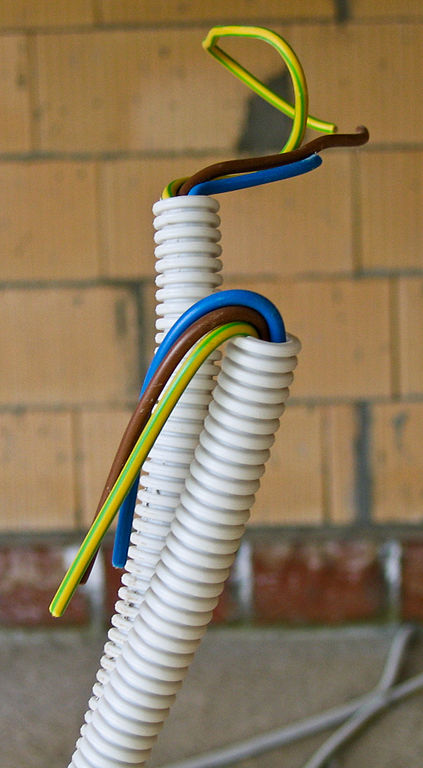
\includegraphics[width=\textwidth,height=0.8\textheight,keepaspectratio]{a19/ElectricWireGrounded.jpg}\\
    {\tiny \hyperlink{refs}{\cite{wm}}}
  \end{center}
\end{frame}

\begin{frame}
  \frametitle{DIN VDE 0100 auch DIN 57100}
  \begin{center} \large
    \begin{tabular}{c|c|c}
      Schutzleiter & Außenleiter & Neutralleiter \\ \hline \hline
      Grüngelb & Braun & Blau \\
    \end{tabular}
  \end{center}
\end{frame}

\section*{Die Erdung von Antennen}

\begin{frame}
  \frametitle{Die Erdung von Antennen}
  \begin{center}
    \begin{block}{DIN VDE 0855 Teil 300}
      Antennenanlagen außerhalb von Gebäuden müssen geerdet werden. Dazu müssen sie mit dem Erdungsleiter des Gebäudes verbunden werden. \\
      Als geeigneter Erdungsleiter gilt ein Einzelmassivdraht mit einem Mindestquerschnitt von $16 mm^2$ Kupfer, isoliert oder blank, oder $25 mm^2$ Aluminium isoliert oder $50 mm^2$ Stahl.
    \end{block}
  \end{center}
\end{frame}

\begin{frame}
  \frametitle{Erdungsschelle}
  \begin{center}
    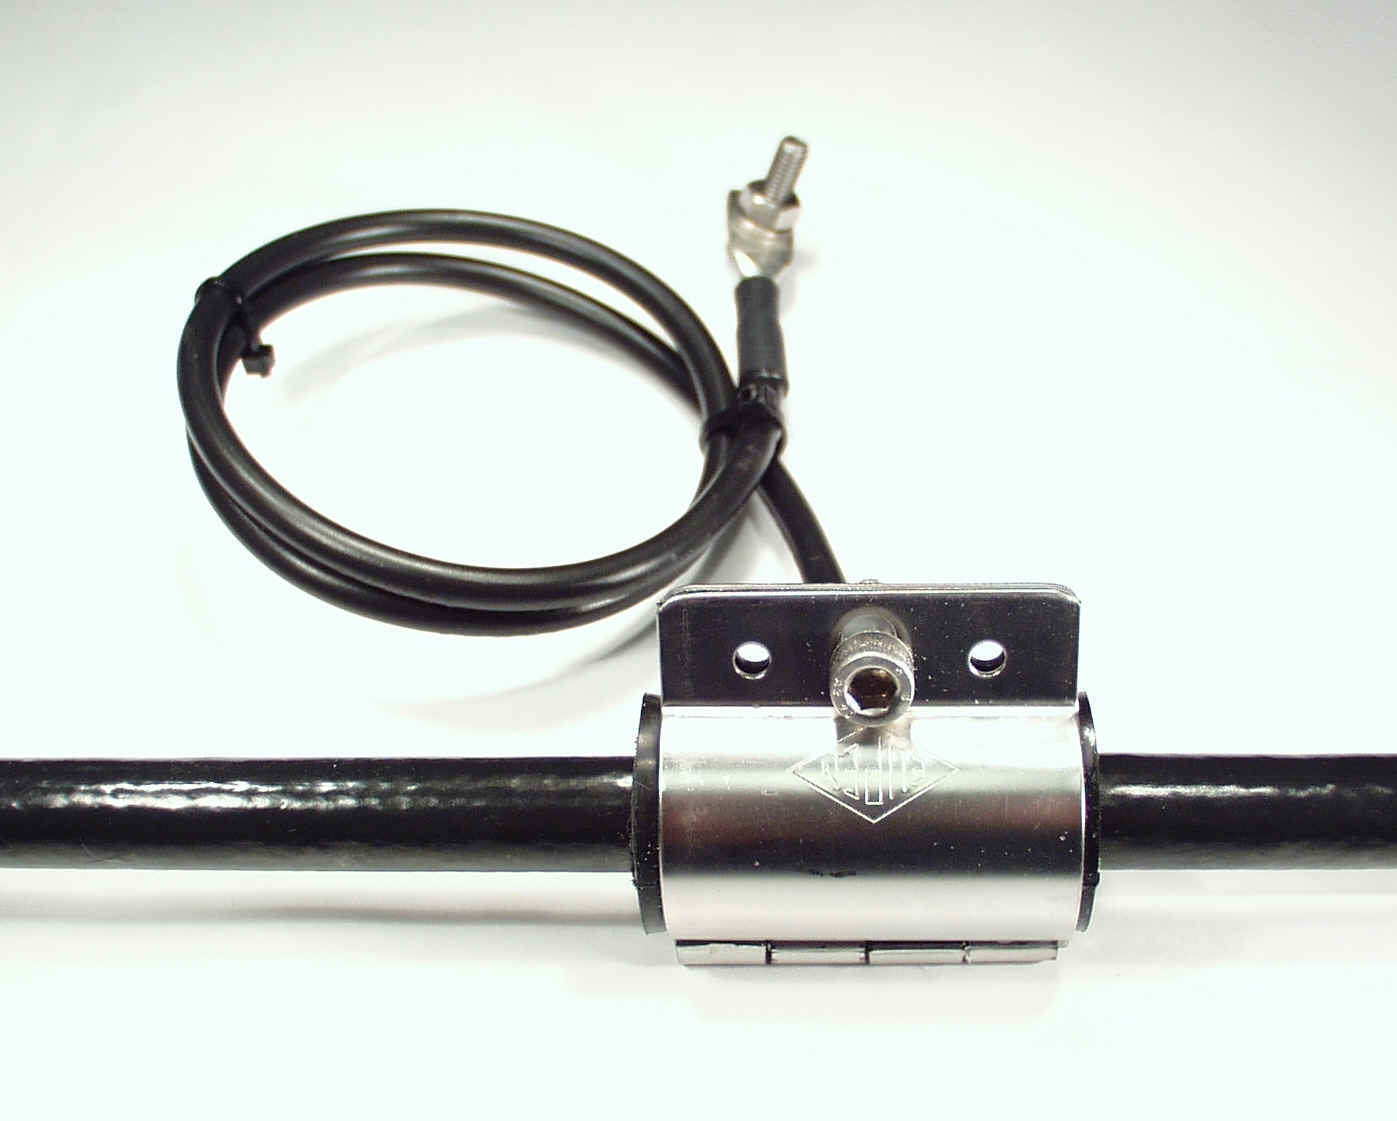
\includegraphics[width=\textwidth,height=0.8\textheight,keepaspectratio]{a19/AntenneErden.jpg}\\
    \tiny Erdungsschelle \url{http://www.kabel-kusch.de/ERDUNG/erdung.htm} \\[1em]
  \end{center}
\end{frame}

\section*{Sendeanlage im KFZ}

\begin{frame}
  \frametitle{Sendeanlage im KFZ}
  \begin{center}
    \begin{exampleblock}{TL306}
      Beim Einbau von Sende und/oder Empfangseinrichtungen sind die Anweisungen des KFZ-Herstellers zu beachten
    \end{exampleblock}
    \begin{exampleblock}{TL307}
      Das Antennenkabel ist möglichst weit entfernt von der Fahrzeugverkabelung zu führen.
    \end{exampleblock}
  \end{center}
\end{frame}

\begin{frame}
  \frametitle{Gut zu Wissen}
  \begin{center}
    \begin{block}{Nichtanwendbarkeit des Handyverbots nach StVO §23 Abs. 1a auf lizenzierte Funkamateure}
      Die StVO §23 Abs. 1a (Verbot der Handybenutzung während der Fahrt ohne Freisprecheinrichtung) bezieht sich nur auf Mobilfunkbenutzer und auf öffentliche Netze. Gemäß aktuellen deutschen Telekommunikationsgesetzen zählen Benutzer von Betriebsfunksystemen wie auch Funkamateure nicht zu diesem Personenkreis. Die StVO §23 Abs. 1a ist somit nicht auf Amateurfunkgeräte anwendbar.
    \end{block}
  \end{center}
\end{frame}

\section*{Personenschutz}

\begin{frame}
  \frametitle{Sicherheitsabstand}
  \begin{center}
    \begin{block}{Sicherheitsabstand zu Antennen in $m$}
      $$d = \frac{\sqrt{30\Omega \cdot P_{EIRP}}}{E}$$ \\[3em]
      \begin{center}
        $E$ nach ICNIRP DIN VDE 0848 \\[1em]
        \begin{tabular}{c|c}
          Frequenz & $E$ in $\frac{V}{m}$ \\ \hline \hline
          unter 10\,MHz & $E = 87 / \sqrt{f_{MHz}}$ \\ \hline
          10\,MHz--400\,MHz & $E = 27,5$ \\ \hline
          400\,MHz--2\,GHz & $E = 1,375 \cdot \sqrt{f_{MHz}}$ \\ \hline
          über 2\,GHz & $E = 61$
        \end{tabular}
      \end{center}
    \end{block}
  \end{center}
  Siehe auch \url{http://emf3.bundesnetzagentur.de/grenzwerte.html}
\end{frame}

\begin{frame}
  \frametitle{Sicherheitsabstand}
  \begin{center}
    \begin{block}{Reduzierungsfaktor}
      \begin{center}
        \begin{tabular}{c|c}
          Betriebsart & Faktor \\ \hline \hline
          SSB & $1:6 = 0,167$ \\ \hline
          CW & $1:4 = 0,25$ \\ \hline
          FM & $1$ \\ \hline
          Digimodes & $1$
        \end{tabular} \end{center}
      \end{block}
    \end{center}
  \end{frame}

\section*{Große Station}

\begin{frame}
  \frametitle{Blockschaltbild}
  \begin{center}
    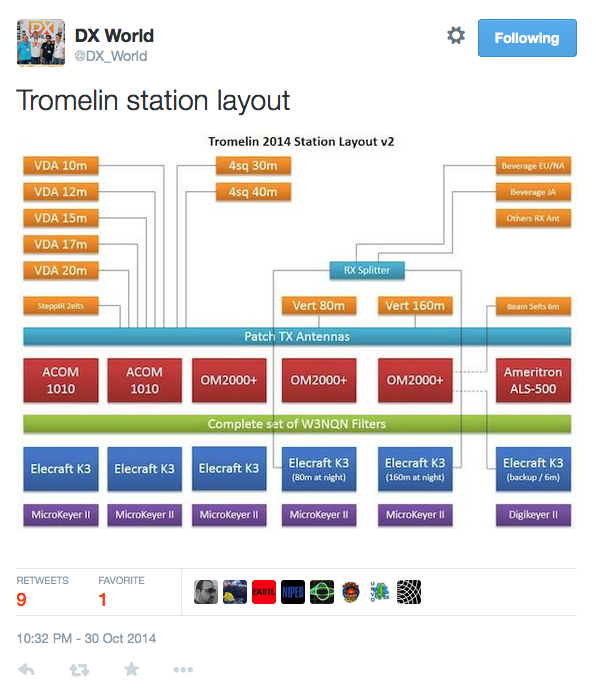
\includegraphics[width=\textwidth,height=0.8\textheight,keepaspectratio]{a19/BsB.png}\\
    {\tiny Tromelin DX FT4TA \url{https://twitter.com/DX_World/status/527936113197858817?s=03}}
  \end{center}
\end{frame}

\renewcommand{\refname}{Referenzen}

\hypertarget{refs}{}
\textcolor{white}{} \\ %\vspace{} geht nicht
\Large Referenzen/Links
\footnotesize

\begin{thebibliography}{}
    \bibitem{darc}  DARC Online-Lehrgang Lektion A19:
                    \url{https://www.darc.de/der-club/referate/ajw/lehrgang-ta/a19/}
    \bibitem{wm} 	Wikimedia:
                    \url{https://commons.wikimedia.org/wiki/File:Regtp_Antennenwagen.jpg}
                    \url{https://upload.wikimedia.org/wikipedia/commons/thumb/0/00/EMI_coupling_modes.svg/1024px-EMI_coupling_modes.svg.png}
                    \url{https://commons.wikimedia.org/wiki/File:ElectricWireGrounded.jpg}
    \bibitem{beam}  Youtube:
                    \url{https://www.youtube.com/watch?v=yLpVnguqwLY}
    \bibitem{wp}    Wikipedia - Die freie Enzyklopädie:
                    \url{https://de.wikipedia.org/wiki/Elektrisches_Feld}
	\bibitem{bna}   Fragenkatalog Bundesnetzagentur Technik Klasse A:
                    \url{https://www.bundesnetzagentur.de/SharedDocs/Downloads/DE/Sachgebiete/Telekommunikation/Unternehmen_Institutionen/Frequenzen/Amateurfunk/Fragenkatalog/TechnikFragenkatalogKlasseAf252rId9014pdf.pdf?__blob=publicationFile&v=3}
\end{thebibliography}

% Hier könnte noch eine Kontaktfolie stehen

\end{document}

